\documentclass[11pt,a4paper,oneside]{report}

% ============================================================
% Encoding, typography, and layout
% ============================================================
\usepackage[T1]{fontenc}
\usepackage[utf8]{inputenc}
\usepackage{lmodern}
\usepackage[
  a4paper,
  top=2.35cm,
  bottom=2.45cm,
  left=2.35cm,
  right=2.35cm,
  headheight=22pt,
  headsep=0.45cm,
  footskip=0.90cm
]{geometry}
\usepackage{microtype}
\usepackage{parskip}
\usepackage{needspace}
\usepackage{setspace}

% ============================================================
% Mathematics
% ============================================================
\usepackage{amsmath}
\usepackage{amssymb}
\usepackage{mathtools}

% ============================================================
% Tables, lists, and code
% ============================================================
\usepackage{booktabs}
\usepackage{tabularx}
\usepackage{array}
\usepackage{longtable}
\usepackage{enumitem}
\usepackage{listings}

% ============================================================
% Graphics
% ============================================================
\usepackage{graphicx}
\usepackage[table]{xcolor}
\usepackage{float}
\graphicspath{{./}}
\usepackage{tikz}
\usetikzlibrary{
  arrows.meta,
  positioning,
  fit,
  calc,
  shapes.geometric,
  backgrounds
}
\usepackage{pgfplots}
\pgfplotsset{compat=1.18}

% ============================================================
% Colour, boxes, headings, captions, navigation
% ============================================================
\usepackage[most]{tcolorbox}
\usepackage{titlesec}
\usepackage{caption}
\usepackage{fancyhdr}
\usepackage{hyperref}

% ============================================================
% Palette
% ============================================================
\definecolor{SapienzaRed}{RGB}{145,31,52}
\definecolor{DeepGreen}{RGB}{24,112,60}
\definecolor{RemarkGray}{RGB}{78,78,78}
\definecolor{SoftBlueGray}{RGB}{245,247,250}
\definecolor{SoftGreen}{RGB}{244,249,245}
\definecolor{SoftGray}{RGB}{247,247,247}
\definecolor{SoftRed}{RGB}{251,246,247}
\definecolor{TableTint}{RGB}{248,240,242}
\definecolor{LinkColor}{RGB}{100,20,38}
\definecolor{ThreatTint}{RGB}{252,242,244}
\definecolor{ProtectTint}{RGB}{241,248,243}

% ============================================================
% Global typography
% ============================================================
\setlength{\parindent}{0pt}
\setlength{\parskip}{0.52em}
\linespread{1.03}
\renewcommand{\arraystretch}{1.18}
\setlist[itemize]{leftmargin=1.55em,itemsep=0.22em,topsep=0.34em}
\setlist[enumerate]{leftmargin=1.78em,itemsep=0.25em,topsep=0.34em}

\titleformat{\chapter}[display]
  {\normalfont}
  {\color{SapienzaRed}\large\bfseries\MakeUppercase{Chapter \thechapter}}
  {0.25em}
  {\Huge\bfseries}
  [\vspace{0.35em}{\color{SapienzaRed}\titlerule[0.8pt]}]
\titlespacing*{\chapter}{0pt}{-0.7cm}{1.15cm}

\titleformat{\section}
  {\normalfont\Large\bfseries}
  {\thesection}{0.72em}{}
\titleformat{\subsection}
  {\normalfont\large\bfseries}
  {\thesubsection}{0.66em}{}
\titleformat{\subsubsection}
  {\normalfont\normalsize\bfseries}
  {\thesubsubsection}{0.60em}{}
\titlespacing*{\section}{0pt}{1.35em}{0.58em}
\titlespacing*{\subsection}{0pt}{1.05em}{0.40em}
\titlespacing*{\subsubsection}{0pt}{0.90em}{0.32em}

% ============================================================
% Hyperlinks
% ============================================================
\hypersetup{
  colorlinks=true,
  linkcolor=LinkColor,
  urlcolor=LinkColor,
  citecolor=LinkColor,
  pdfauthor={Matt Clifford Trinidad Ramos},
  pdftitle={Security in Software Applications -- Lecture Notes}
}

% ============================================================
% Header and footer
% ============================================================
\pagestyle{fancy}
\fancyhf{}
\renewcommand{\chaptermark}[1]{\markboth{#1}{}}
\renewcommand{\sectionmark}[1]{\markright{#1}}
\fancyhead[L]{\small\nouppercase{\leftmark}}
\fancyhead[R]{\small\nouppercase{\rightmark}}
\fancyfoot[L]{\small Security in Software Applications}
\fancyfoot[C]{\small \thepage}
\fancyfoot[R]{\small Matt Clifford Trinidad Ramos}
\renewcommand{\headrulewidth}{0.45pt}
\renewcommand{\footrulewidth}{0.45pt}
\renewcommand{\headrule}{\hbox to\headwidth{\color{SapienzaRed}\leaders\hrule height \headrulewidth\hfill}}
\renewcommand{\footrule}{\hbox to\headwidth{\color{SapienzaRed}\leaders\hrule height \footrulewidth\hfill}}

\fancypagestyle{plain}{%
  \fancyhf{}
  \fancyfoot[L]{\small Security in Software Applications}
  \fancyfoot[C]{\small \thepage}
  \fancyfoot[R]{\small Matt Clifford Trinidad Ramos}
  \renewcommand{\headrulewidth}{0pt}
  \renewcommand{\footrulewidth}{0.45pt}
  \renewcommand{\footrule}{\hbox to\headwidth{\color{SapienzaRed}\leaders\hrule height \footrulewidth\hfill}}
}

% ============================================================
% Semantic boxes -- intentionally restrained
% ============================================================
\newtcolorbox{definitionbox}[1]{
  enhanced,
  breakable,
  colback=SoftBlueGray,
  colframe=SapienzaRed,
  colbacktitle=SapienzaRed,
  coltitle=white,
  title={Definition -- #1},
  fonttitle=\bfseries,
  boxrule=0.65pt,
  arc=1.4mm,
  left=2mm,right=2mm,top=1.4mm,bottom=1.4mm
}

\newtcolorbox{keyconcept}{
  enhanced,
  breakable,
  colback=SoftGreen,
  colframe=DeepGreen,
  colbacktitle=DeepGreen,
  coltitle=white,
  title={Key Concept},
  fonttitle=\bfseries,
  boxrule=0.65pt,
  arc=1.4mm,
  left=2mm,right=2mm,top=1.4mm,bottom=1.4mm
}

\newtcolorbox{remarkbox}[1]{
  enhanced,
  breakable,
  colback=SoftGray,
  colframe=RemarkGray,
  colbacktitle=RemarkGray,
  coltitle=white,
  title={Remark -- #1},
  fonttitle=\bfseries,
  boxrule=0.60pt,
  arc=1.4mm,
  left=2mm,right=2mm,top=1.4mm,bottom=1.4mm
}

\newtcolorbox{examplebox}[1]{
  enhanced,
  breakable,
  colback=SoftRed,
  colframe=SapienzaRed,
  colbacktitle=white,
  coltitle=SapienzaRed,
  title={Example -- #1},
  fonttitle=\bfseries,
  boxrule=0.60pt,
  arc=1.4mm,
  left=2mm,right=2mm,top=1.4mm,bottom=1.4mm
}

% ============================================================
% Captions and listings
% ============================================================
\captionsetup{font=small,labelfont=bf,justification=centering}

\lstdefinestyle{coursecode}{
  basicstyle=\ttfamily\small,
  columns=fullflexible,
  keepspaces=true,
  frame=single,
  framerule=0.4pt,
  rulecolor=\color{RemarkGray},
  backgroundcolor=\color{SoftGray},
  xleftmargin=0.8em,
  xrightmargin=0.8em,
  aboveskip=0.8em,
  belowskip=0.8em,
  showstringspaces=false,
  breaklines=true,
  breakatwhitespace=false,
  tabsize=4
}
\lstset{style=coursecode}

% ============================================================
% TikZ styles
% ============================================================
\tikzset{
  sbox/.style={
    draw=RemarkGray,
    fill=white,
    rounded corners=1.2mm,
    minimum height=9mm,
    align=center,
    font=\small,
    inner xsep=5mm,
    inner ysep=2mm
  },
  threatbox/.style={sbox,draw=SapienzaRed,fill=ThreatTint},
  protectbox/.style={sbox,draw=DeepGreen,fill=ProtectTint},
  arrow/.style={-{Latex[length=2mm]},thick,draw=RemarkGray},
  badarrow/.style={-{Latex[length=2mm]},thick,draw=SapienzaRed},
  goodarrow/.style={-{Latex[length=2mm]},thick,draw=DeepGreen},
  dasharrow/.style={-{Latex[length=2mm]},thick,dashed,draw=RemarkGray}
}

\newcolumntype{Y}{>{\raggedright\arraybackslash}X}
\newcolumntype{L}[1]{>{\raggedright\arraybackslash}p{#1}}
\newcolumntype{C}[1]{>{\centering\arraybackslash}p{#1}}

% All course figures are included in the project folder.
\newcommand{\courseimage}[2]{%
  \includegraphics[width=#1]{#2}%
}

% ============================================================
% Document
% ============================================================
\begin{document}

% ------------------------------------------------------------
% Title page
% ------------------------------------------------------------
\hypersetup{pageanchor=false}
\begin{titlepage}
\thispagestyle{empty}
\centering

\vspace*{1.35cm}

{\color{SapienzaRed}\rule{0.84\textwidth}{0.9pt}}

\vspace{0.82cm}

{\LARGE\bfseries\MakeUppercase{Security in Software Applications}\par}

\vspace{0.36cm}

{\Large Lecture Notes\par}

\vspace{0.82cm}

{\color{SapienzaRed}\rule{0.84\textwidth}{0.9pt}}

\vspace{1.25cm}


\includegraphics[width=0.65\textwidth,trim=20bp 210bp 20bp 210bp,clip]{sapienza_logo.png}

\vfill

{\small\textsc{Lecturer}\par}
\vspace{0.12cm}
{\large Daniele Friolo\par}

\vspace{0.70cm}

{\small Department of Computer Science\par}
{\small Sapienza University of Rome\par}

\vspace{1.35cm}

{\small\textsc{Notes prepared by}\par}
\vspace{0.12cm}
{\large\bfseries Matt Clifford Trinidad Ramos\par}

\vfill
\end{titlepage}
\hypersetup{pageanchor=true}
\pagenumbering{arabic}
\setcounter{page}{1}

\tableofcontents
\clearpage

% ============================================================
\chapter{Foundations of Software Security}
\label{chap:foundations}
% ============================================================

Software security studies how software contributes both to protection and to failure. Modern systems depend on software to enforce authentication, access control, cryptographic protocols, isolation, and many other security mechanisms, yet the same software can expose unintended behavior that an adversary can deliberately trigger. The engineering objective is therefore not simply to add ``security features,'' but to control the risks created by the complete behavior of the system.

\section{Security as an Engineering Property}
\label{sec:engineering-property}

A computer system may be a conventional server or desktop, a mobile device, an embedded controller, a cloud service, or an industrial control system. Despite their differences, these systems share two security-relevant characteristics: they combine hardware and software, and they interact with an external environment containing inputs, users, networks, devices, and other systems that cannot all be assumed trustworthy.

\begin{definitionbox}{Software Security}
Software security is the discipline of managing security risks created by software: understanding the threats and vulnerabilities that can make software unsafe, and applying principles, methods, and technologies that reduce those risks.
\end{definitionbox}

Security differs from ordinary correctness because an adversary actively searches for behavior that violates a security objective. A fault may be triggered accidentally; an attack is deliberately constructed around the capabilities available to an attacker.

\subsection{Functional and Security Properties}

Functional properties describe what a system should do. Security properties also constrain what it must \emph{not} do, especially when it receives malformed or maliciously crafted input.

Consider a compressor and decompressor. A natural functional property is

\begin{equation}
\operatorname{Uncompress}(\operatorname{Compress}(f)) = f.
\label{eq:compress-correctness}
\end{equation}

This checks expected use. A security-oriented property must additionally consider inputs that were not generated by the compressor. If a byte sequence \(C\) is not a valid encoding of any file under the expected format, the decompressor should fail safely rather than enter undefined or dangerous behavior:

\begin{equation}
C \notin \operatorname{Range}(\operatorname{Compress})
\quad\Longrightarrow\quad
\operatorname{Uncompress}(C)=\operatorname{Error}.
\label{eq:malicious-input}
\end{equation}

The second property is harder because it quantifies over arbitrary, potentially hostile input rather than over values produced by a trusted producer.

\begin{keyconcept}
Correctness under expected inputs is not enough for security. Secure software must also constrain behavior under malformed, unexpected, and adversarial inputs.
\end{keyconcept}

\subsection{Programming Background and Safety-Relevant Semantics}

Several examples in this material rely on low-level C/C++ memory management, Java run-time checks, and object-oriented visibility rules. These constructs are not merely syntactic prerequisites: they determine which safety properties the language or runtime enforces automatically and which remain the programmer's responsibility.

Consider a typical C string-copying fragment:

\begin{lstlisting}[language=C,caption={A C string-copying fragment whose allocation is one byte too small.},label={lst:warmup-copy}]
char *copying_a_string(char *a) {
    char *b = malloc(strlen(a));
    strcpy(b, a);
    return b;
}
\end{lstlisting}

As written, the allocation reserves space for the visible characters but not for the terminating null byte copied by \texttt{strcpy}. A corrected allocation must reserve at least \texttt{strlen(a) + 1} bytes and must also check the result of \texttt{malloc}. The example illustrates how a seemingly ordinary programming idiom can already depend on exact API and representation semantics.

Pointer arithmetic provides another C-specific source of responsibility. An expression such as \texttt{*(p++)} both dereferences the current pointer and advances it; the language does not automatically prove that the new pointer remains within the intended array object. A representative loop is:

\begin{lstlisting}[language=C,caption={Pointer arithmetic over a four-element integer array.}]
int using_pointer_arithmetic(int pin[]) {
    int sum = 0;
    int *pointer = pin;
    for (int i = 0; i < 4; i++) {
        sum += *pointer;
        pointer++;
    }
    return sum;
}
\end{lstlisting}

Java moves several of these checks into the runtime. A corresponding array loop can be written as:

\begin{lstlisting}[language=Java,caption={A Java array loop with run-time bounds checks.}]
public int summingAnArray(int[] pin) {
    int sum = 0;
    for (int i = 0; i < 4; i++) {
        sum += pin[i];
    }
    return sum;
}
\end{lstlisting}

Array accesses are bounds-checked and can raise
\texttt{ArrayIndexOutOfBoundsException}; dereferencing \texttt{null}
raises \texttt{NullPointerException}. Visibility modifiers such as
\texttt{private}, \texttt{protected}, and \texttt{public}, together
with \texttt{final}, also constrain which code can access or modify
state. These mechanisms do not make software automatically secure,
but they change the classes of errors that can occur silently.

\section{Threat Models and Adversaries}
\label{sec:threat-models}

Security reasoning starts by identifying the assets that matter, the actors who may attack them, the capabilities available to those actors, and the actions that would count as a security violation. Without this context, the statement ``the system is secure'' is underspecified.

\begin{definitionbox}{Threat Model}
A threat model describes the adversaries and attack conditions considered relevant: what the attacker can access, control, observe, modify, or impersonate, and which assets and security properties must be protected.
\end{definitionbox}

The distinction between a deliberate adversary and an accidental hazard separates security from ordinary safety and fault tolerance. A threat model may include external attackers, malicious insiders, compromised clients, or other principals capable of intentionally selecting inputs or actions that exploit weaknesses.

\begin{remarkbox}{The word ``threat'' is overloaded}
Security writing uses \emph{threat} in at least two closely related senses: the actor or source of danger, and a class of adverse actions such as spoofing or denial of service. In this document, the surrounding context makes the intended meaning explicit; a threat is never treated as the software vulnerability itself.
\end{remarkbox}

\subsection{Assets, Threats, Vulnerabilities, and Risk}

An \emph{asset} is something a stakeholder values, such as information, functionality, availability of a service, or control over a system. A \emph{threat} is a potential cause of harm. A \emph{vulnerability} is a security-relevant weakness that can be exploited. \emph{Risk} captures the possibility and consequences of harmful outcomes when threats can reach vulnerable assets.

\begin{figure}[htbp]
\centering
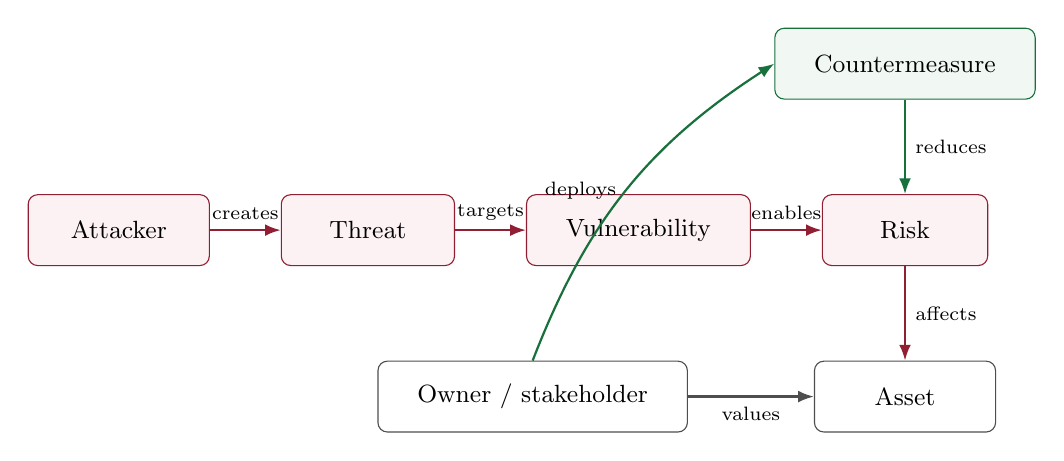
\begin{tikzpicture}[node distance=10mm and 9mm]
  \node[threatbox, minimum width=2.3cm] (attacker) {Attacker};
  \node[threatbox, right=of attacker, minimum width=2.2cm] (threat) {Threat};
  \node[threatbox, right=of threat, minimum width=2.7cm] (vuln) {Vulnerability};
  \node[threatbox, right=of vuln, minimum width=2.1cm] (risk) {Risk};

  \node[sbox, below=12mm of risk, minimum width=2.3cm] (asset) {Asset};
  \node[sbox, left=16mm of asset, minimum width=2.9cm] (owner) {Owner / stakeholder};
  \node[protectbox, above=12mm of risk, minimum width=2.8cm] (counter) {Countermeasure};

  \draw[badarrow] (attacker) -- node[above,font=\scriptsize]{creates} (threat);
  \draw[badarrow] (threat) -- node[above,font=\scriptsize]{targets} (vuln);
  \draw[badarrow] (vuln) -- node[above,font=\scriptsize]{enables} (risk);
  \draw[badarrow] (risk) -- node[right,font=\scriptsize]{affects} (asset);

  \draw[arrow] (owner) -- node[below,font=\scriptsize]{values} (asset);
  \draw[goodarrow] (owner.north) to[bend left=18] node[left,font=\scriptsize]{deploys} (counter.west);
  \draw[goodarrow] (counter) -- node[right,font=\scriptsize]{reduces} (risk);
\end{tikzpicture}
\caption{A compact causal view of software-security risk. Countermeasures are introduced to reduce the risk that threats exploit vulnerabilities and harm valued assets.}
\label{fig:risk-chain}
\end{figure}

A security policy specifies the security requirements that the system is expected to enforce. The policy must therefore make clear both \emph{what} is being protected and \emph{against whom or what} it is being protected.

\section{Security Objectives}
\label{sec:objectives}

The most widely used high-level objectives are confidentiality, integrity, and availability, commonly abbreviated as CIA.

\begin{table}[htbp]
\centering
\caption{Core security objectives.}
\label{tab:cia}
\begin{tabularx}{0.90\textwidth}{>{\bfseries}L{3.0cm} Y}
\toprule
\rowcolor{TableTint}
Objective & Meaning \\
\midrule
Confidentiality & Information is not disclosed to unauthorised parties. \\
Integrity & Information or system state is not modified in an unauthorised manner. \\
Availability & Authorised users can access required information or functionality when needed. \\
\bottomrule
\end{tabularx}
\end{table}

Other useful goals include authentication, authorisation, accountability, non-repudiation, auditing, privacy, anonymity, multi-level security, continuous monitoring, and assurance. Traceability and auditing support forensic reconstruction after an incident, while monitoring provides a real-time view of security-relevant activity. Assurance is a meta-property: it concerns the evidence that the stated security goals are actually met. These goals are related but distinct. In particular, \emph{authentication} is not the ``A'' in CIA: it establishes identity, whereas availability concerns continued access to information or service.

Integrity can be more important than secrecy in many settings. A bank balance, a medical record, or executable software may be public or observable in some contexts, but unauthorised modification can still be catastrophic. Availability may also conflict with privacy goals when the desired outcome is to make information inaccessible.

\subsection{From Threats to Requirements}

Different threat classes motivate different security requirements.

\begin{table}[htbp]
\centering
\caption{Examples of threats and the security requirements they motivate.}
\label{tab:threat-requirement}
\begin{tabularx}{0.82\textwidth}{Y Y}
\toprule
\rowcolor{TableTint}
\textbf{Threat} & \textbf{Primary requirement} \\
\midrule
Information disclosure & Confidentiality \\
Tampering with information & Integrity \\
Denial of service & Availability \\
Spoofing / identity impersonation & Authentication \\
Unauthorised operations & Access control / authorisation \\
\bottomrule
\end{tabularx}
\end{table}

\section{Bugs, Vulnerabilities, Exploits, and Malware}
\label{sec:bug-vuln-exploit}

Terminology matters because related concepts describe different stages of a security failure.

\begin{definitionbox}{Bug / Flaw}
A bug or flaw is a defect in specification, design, implementation, configuration, or transformation that causes the system to behave incorrectly or less robustly than intended.
\end{definitionbox}

\begin{definitionbox}{Vulnerability}
A vulnerability is a security-relevant weakness that can be reached and used to violate a security policy under an applicable threat model.
\end{definitionbox}

\begin{definitionbox}{Exploit}
An exploit is a concrete technique, input, command sequence, or program that deliberately takes advantage of a vulnerability to trigger unintended behavior.
\end{definitionbox}

Malware is malicious software designed to compromise a system, disrupt operation, steal information, or otherwise violate policy. Malware may use one or more exploits, but malware and exploit are not synonyms.

\begin{figure}[htbp]
\centering
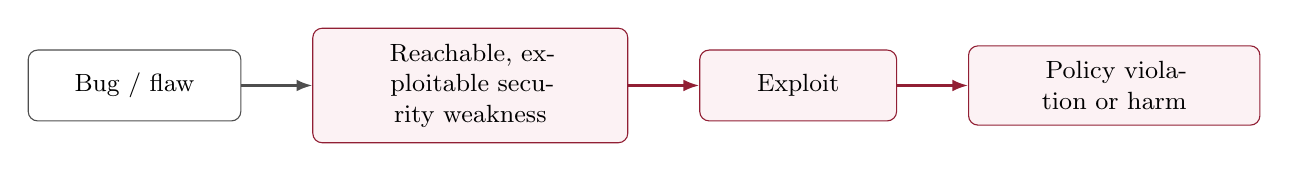
\begin{tikzpicture}[node distance=9mm]
  \node[sbox, minimum width=2.7cm] (flaw) {Bug / flaw};
  \node[threatbox, right=of flaw, minimum width=3.5cm, text width=3.0cm] (vuln) {Reachable, exploitable security weakness};
  \node[threatbox, right=of vuln, minimum width=2.5cm] (exploit) {Exploit};
  \node[threatbox, right=of exploit, minimum width=3.2cm, text width=2.7cm] (impact) {Policy violation or harm};

  \draw[arrow] (flaw) -- (vuln);
  \draw[badarrow] (vuln) -- (exploit);
  \draw[badarrow] (exploit) -- (impact);
\end{tikzpicture}
\caption{A bug becomes security-relevant when it is reachable and exploitable; an exploit is the concrete mechanism used to trigger the vulnerability.}
\label{fig:defect-chain}
\end{figure}

A flaw can exist without a known practical exploit. Conversely, multiple exploits can target the same underlying vulnerability. A threat describes danger or an adversarial class; it is not itself the software weakness.

\subsection{Where Software Flaws Enter the System}

Security-relevant defects can be introduced at several levels. A \emph{design flaw} is created while deciding how the system should work; a \emph{code-level flaw} is introduced while implementing that design. Configuration mistakes, unsafe user choices, and unforeseen consequences of intended functionality can also create vulnerabilities even when the code follows its nominal specification.

Implementation defects can be divided usefully into two groups. Some can be understood directly from the program---for example typographical mistakes, confusing variables, off-by-one errors, invalid array access, or incorrect control logic. Others arise from interaction with the underlying platform or another system, including buffer overflow, integer overflow or underflow, SQL injection, cross-site scripting, and cross-site request forgery.

\begin{table}[htbp]
\centering
\caption{Representative points at which security flaws can enter a software system.}
\label{tab:flaw-sources}
\begin{tabularx}{\textwidth}{>{\bfseries}L{3.2cm} Y}
\toprule
\rowcolor{TableTint}
Source & Typical interpretation \\
\midrule
Design & The architecture or specification permits an unsafe behavior or omits a required control. \\
Implementation & The design may be sound, but the code contains logic, memory, arithmetic, validation, or API-use defects. \\
Configuration & Deployment choices expose unsafe defaults, excessive privilege, unnecessary services, or weak policy. \\
User interaction & A user can select insecure options, disclose credentials, or exercise functionality in an unsafe way. \\
Unforeseen functionality & Intended features interact in ways that create abuse cases not considered during design. \\
\bottomrule
\end{tabularx}
\end{table}

\subsection{Worked Example: Three Different Security Defects}

The following small balance-management routine contains defects at three different abstraction levels:

\begin{lstlisting}[language=C,caption={A balance-management routine with logic, validation, and integer-arithmetic defects.},label={lst:balance-flaws}]
int balance;

void decrease(int amount) {
    if (balance <= amount)
        balance = balance - amount;
    else
        printf("Insufficient funds\n");
}

void increase(int amount) {
    balance = balance + amount;
}
\end{lstlisting}

First, the sufficient-balance test is reversed: the intended check for allowing a withdrawal is conceptually \texttt{balance >= amount}. This is a local logic error that can be found by inspecting the code. Second, the interface does not specify or validate what should happen when \texttt{amount} is negative; this is an input-validation problem whose boundary between design and implementation depends on where the contract should have been established. Third, \texttt{balance + amount} can overflow the representation of \texttt{int}; this defect depends on the semantics of the underlying integer type and execution platform.

\subsection{Different Targets Require Different Defenses}

A useful distinction is to ask what the defensive mechanism is trying to reduce. Tools such as antivirus software, intrusion detection, and firewalls primarily detect or block concrete exploit activity. Forensics, policy, incentives, and deterrence can address the actors and conditions that create threats. Eliminating vulnerabilities requires engineering the software and its configuration so that the exploitable weakness is removed or constrained.

\begin{table}[htbp]
\centering
\caption{Different defensive targets require different mechanisms.}
\label{tab:defense-targets}
\begin{tabularx}{0.94\textwidth}{>{\bfseries}L{3.0cm} Y}
\toprule
\rowcolor{TableTint}
Target & Representative response \\
\midrule
Exploit activity & Antivirus, intrusion detection, firewalls, runtime blocking, incident response. \\
Threat actor / threat conditions & Forensics, policy, incentives, deterrence, access governance. \\
Underlying vulnerability & Secure design, secure implementation, validation, patching, safer abstractions, verification. \\
\bottomrule
\end{tabularx}
\end{table}

\section{Attack Surfaces and Historical Perspective}
\label{sec:attack-surface}

Connectivity expands the attack surface. Software may be reachable directly over a network, or it may process untrusted data obtained through files, messages, media formats, USB devices, web requests, or other interfaces. As software becomes more connected, application, operating-system, and network security become increasingly interdependent.

Viruses and worms illustrate this distinction. A virus typically attaches to or modifies a host program and spreads when infected code runs. A worm is a standalone self-propagating program that can spread across machines without requiring a user to execute an infected host file.

The 1988 Morris worm became an early demonstration of how software vulnerabilities could propagate across the Internet. SQL Slammer provided a later example of extremely rapid network propagation in January 2003. These incidents are useful not because their specific software environments are still current, but because they demonstrate recurring properties: remotely reachable code, untrusted input, and vulnerabilities that can be automated at network scale.

\begin{figure}[htbp]
\centering
\begin{minipage}{0.47\textwidth}
\centering
\courseimage{\linewidth}{slammer_initial.jpg}\\[-0.1em]
{\scriptsize Early snapshot: no visible infected hosts in the captured view.}
\end{minipage}\hfill
\begin{minipage}{0.47\textwidth}
\centering
\courseimage{\linewidth}{slammer_spread.jpg}\\[-0.1em]
{\scriptsize Later snapshot: widespread global infection activity.}
\end{minipage}
\caption{Historical snapshots of the rapid global propagation of the Sapphire/Slammer worm. The images are retained as qualitative evidence of propagation speed, not as a dataset for quantitative analysis.}
\label{fig:slammer-spread}
\end{figure}

The economics of exploitation also changed the threat environment. Vulnerabilities and reliable exploits can have significant monetary value, creating incentives for professional criminal groups, commercial exploit markets, and state-sponsored actors. Stuxnet is a prominent historical example of the level of resources and engineering that can be associated with state-linked offensive operations. Security engineering must therefore account for attackers with substantial resources rather than assuming only casual experimentation.

\begin{figure}[htbp]
\centering
\courseimage{0.86\textwidth}{zerodium_desktop.png}\\[0.7em]
\courseimage{0.86\textwidth}{zerodium_mobile.png}
\caption{Historical exploit-market payout charts for desktop/server and mobile targets. They illustrate the economic value attached to reliable exploitation; the values are historical and must not be interpreted as current market prices.}
\label{fig:historical-payouts}
\end{figure}

\subsection{Large Attack Surfaces and Recurring ``Lost Battles''}

Several recurring software categories make security particularly difficult. Operating systems expose very large APIs; browsers and email clients process complex, extensible, and often untrusted content; programming languages may leave dangerous memory, formatting, or visibility semantics to the developer; and web applications combine scripting, database interfaces, markup, plug-ins, and network protocols. The more functionality and interfaces a system exposes, the larger the attack surface that must be understood and defended.

The central issue is not that functionality is undesirable. The engineering difficulty is that functionality and convenience often introduce additional states, interfaces, parsers, privileges, and trust assumptions. Security therefore competes for design attention with performance, usability, compatibility, and delivery pressure.

\subsection{Representative Vulnerabilities}

Vulnerabilities recur across very different software platforms. Table~\ref{tab:vuln-examples} collects representative examples from routers, multimedia software, desktop operating systems, web applications, and videoconferencing systems.

\begin{table}[htbp]
\centering
\small
\setlength{\tabcolsep}{3.5pt}
\caption{Representative software vulnerabilities across different platforms.}
\label{tab:vuln-examples}
\begin{tabularx}{\textwidth}{L{2.30cm} L{2.55cm} C{1.05cm} C{1.85cm} Y}
\toprule
\rowcolor{TableTint}
\textbf{System} & \textbf{Identifier} & \textbf{CVSS} & \textbf{Published} & \textbf{Security lesson} \\
\midrule
Cisco Linksys WRT54GC router & \mbox{CVE-2011-0352} & 7.88 & 2011-01-24 & A long POST value could trigger a buffer overflow in the web-management interface and crash the device. \\
\addlinespace
FFmpeg Vorbis decoder & \mbox{CVE-2010-4705} & 9.3 & 2011-01-24 & Integer-size handling in a multimedia decoder created a remotely reachable integer-overflow condition. \\
\addlinespace
Linux / Windows / macOS USB HID handling & \shortstack[l]{\mbox{CVE-2011-0638}\\\mbox{CVE-2011-0640}\\\mbox{CVE-2011-0639}} & 9.3 & 2011-01-24 & Crafted USB Human Interface Device behavior could cause user-assisted execution of unintended programs. \\
\addlinespace
Mozilla Bugzilla & \mbox{CVE-2010-4568} & 7.5 & 2011-01-28 & Weak randomness in cookies and tokens could undermine account security. \\
\addlinespace
TANDBERG videoconferencing & \mbox{CVE-2011-0354} & -- & 2011-02-02 & A root administrator account with no password exposed privileged remote access. \\
\bottomrule
\end{tabularx}
\end{table}

The lesson is not that these specific historical vulnerabilities dominate current systems; it is that recurring categories such as memory errors, weak randomness, insecure defaults, and unsafe device trust reappear in new software environments. The same pattern is visible in newer execution platforms such as smart-contract systems, where integer and authorization errors have reappeared in a different programming environment.

\section{Weakness in Depth}
\label{sec:weakness-depth}

Applications depend on a large software and hardware stack. A defect in an application can create a vulnerability directly, but the application can also inherit weaknesses from libraries, runtimes, databases, operating-system services, compilers, or lower-level hardware interfaces.

\begin{figure}[htbp]
\centering
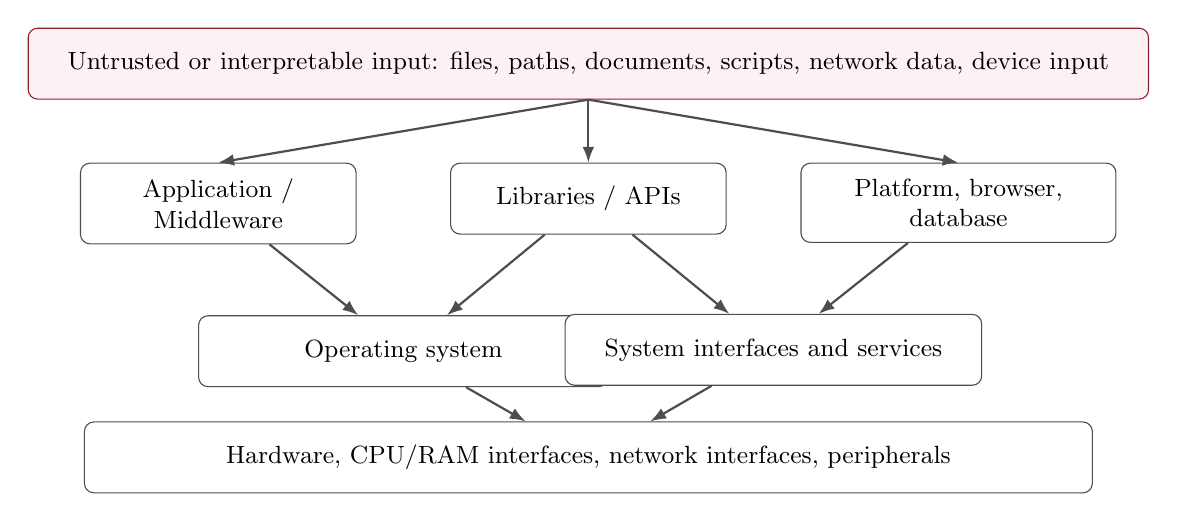
\begin{tikzpicture}[node distance=6mm and 7mm]
  \node[threatbox, minimum width=12.8cm] (input) {Untrusted or interpretable input: files, paths, documents, scripts, network data, device input};

  \node[sbox, below=8mm of input, xshift=-4.7cm, minimum width=3.5cm] (app) {Application /\\Middleware};
  \node[sbox, below=8mm of input, minimum width=3.5cm] (lib) {Libraries / APIs};
  \node[sbox, below=8mm of input, xshift=4.7cm, minimum width=4.0cm] (plat) {Platform, browser,\\database};

  \node[sbox, below=9mm of app, xshift=2.35cm, minimum width=5.2cm] (os) {Operating system};
  \node[sbox, below=9mm of plat, xshift=-2.35cm, minimum width=5.2cm] (api) {System interfaces and services};

  \node[sbox, below=9mm of $(os)!0.5!(api)$, minimum width=12.8cm] (hw) {Hardware, CPU/RAM interfaces, network interfaces, peripherals};

  \draw[arrow] (input.south) -- (app.north);
  \draw[arrow] (input.south) -- (lib.north);
  \draw[arrow] (input.south) -- (plat.north);
  \draw[arrow] (app) -- (os);
  \draw[arrow] (lib) -- (os);
  \draw[arrow] (lib) -- (api);
  \draw[arrow] (plat) -- (api);
  \draw[arrow] (os) -- (hw);
  \draw[arrow] (api) -- (hw);
\end{tikzpicture}
\caption{Software-security weaknesses can arise at multiple layers of the execution stack, from application logic and reusable components to operating-system interfaces and hardware dependencies.}
\label{fig:security-stack}
\end{figure}

This layered view has two consequences. First, a secure application cannot rely blindly on every abstraction below it. Second, infrastructure can simultaneously provide security mechanisms and introduce new attack surfaces.

\subsection{Three Recurring Sources of Vulnerability}

The software stack can create security problems in three broad ways:

\begin{enumerate}
  \item \textbf{Bugs in the application or infrastructure:} a component fails to do what it should do.
  \item \textbf{Inappropriate infrastructure features:} a platform exposes functionality that it should not expose under the intended security policy, often because functionality was prioritized over security.
  \item \textbf{Inappropriate use of legitimate features:} developers misuse a powerful mechanism because its semantics are complex, its secure configuration is non-obvious, or its convenience encourages unsafe defaults.
\end{enumerate}

These categories explain why vulnerability knowledge must be specific to languages, operating systems, databases, frameworks, and application types. The details evolve, but recurring patterns such as input validation failures, injection, unsafe memory operations, and over-permissive interfaces repeatedly reappear.

\section{Trust Beyond Source Code}
\label{sec:trusting-trust}

Security reasoning must include the build and execution toolchain. Source code can appear correct while a compromised compiler, build system, dependency, or binary transformation step injects behavior that is absent from the source.

The classic ``trusting trust'' scenario demonstrates a self-propagating compiler compromise. A malicious compiler can recognize a target program and inject a hidden modification; if it also recognizes that it is compiling a compiler, it can insert the same behavior into the next compiler binary. The malicious logic can therefore persist even after the visible compiler source is cleaned.

\begin{figure}[H]
\centering
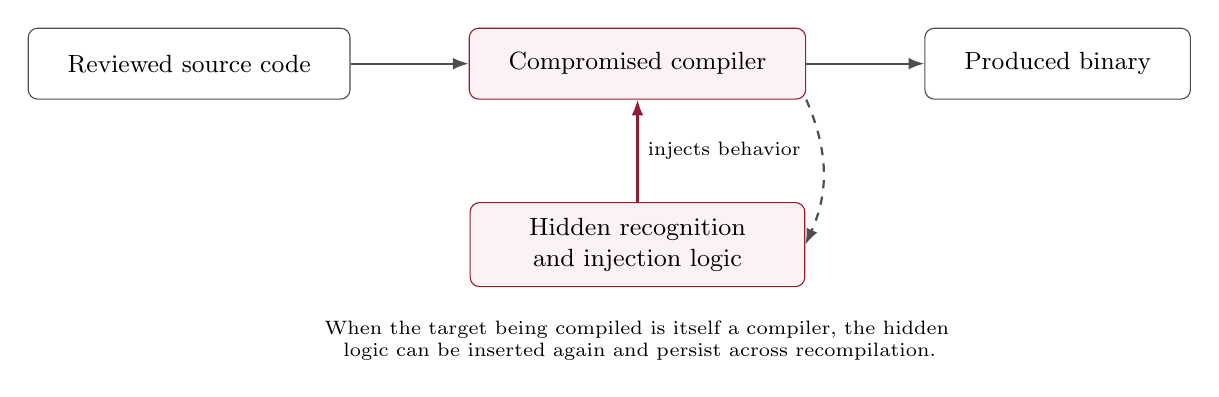
\begin{tikzpicture}[node distance=12mm and 15mm]
  \node[sbox, minimum width=3.6cm] (src) {Reviewed source code};
  \node[threatbox, right=of src, minimum width=3.8cm] (compiler) {Compromised compiler};
  \node[sbox, right=of compiler, minimum width=3.2cm] (binary) {Produced binary};
  \node[threatbox, below=13mm of compiler, minimum width=3.8cm, text width=3.25cm] (hidden) {Hidden recognition and injection logic};

  \draw[arrow] (src) -- (compiler);
  \draw[arrow] (compiler) -- (binary);
  \draw[badarrow] (hidden) -- node[right,font=\scriptsize]{injects behavior} (compiler);
  \draw[dasharrow] (compiler.south east) to[bend left=24] (hidden.east);
  \node[font=\scriptsize, below=3mm of hidden, text width=8.0cm, align=center]
    {When the target being compiled is itself a compiler, the hidden logic can be inserted again and persist across recompilation.};
\end{tikzpicture}
\caption{Source-level review is insufficient if the compiler or wider build chain is not trusted.}
\label{fig:trusting-trust}
\end{figure}

The broader principle is that trust extends transitively through compilers, package managers, libraries, build servers, firmware, and other components used to construct the final program.

\section{Chapter Summary}

Software security is an adversarial form of engineering correctness. It requires a threat model, precise security objectives, a clear distinction among flaws, vulnerabilities, exploits, threats, and risks, and an understanding of how software depends on a wider execution stack. Security is not established by adding isolated features; it is established by controlling behavior across expected and hostile inputs and across every component on which the system depends.

% ============================================================
\chapter{Engineering Secure Software}
\label{chap:engineering}
% ============================================================

Security failures often arise not from one exotic technique but from recurring engineering conditions: incomplete threat awareness, unfamiliar platform semantics, overly permissive interfaces, insecure defaults, and late-stage security review. A robust development process therefore moves security work earlier and distributes it across requirements, design, implementation, testing, and operation.

\section{Awareness, Knowledge, and the Attacker's View}

Two recurring causes of software-security problems are lack of awareness and lack of knowledge. A programmer may know a language well and still be unaware of the security consequences of a library function, integer conversion, parser behavior, browser feature, database interface, or operating-system service.

Functionality and security also create different design pressures. Functionality asks what the program should do; security asks what it must not be allowed to do, including under inputs that no cooperative user would generate. This is why threat discovery requires thinking about how an adversary could misuse legitimate functionality or cross an implicit trust boundary.

Large attack surfaces make this reasoning harder. Operating systems expose large APIs; web browsers support many formats and scripting mechanisms; applications rely on extensive libraries; and low-level languages can place substantial memory-safety responsibility on the programmer. Complexity increases the number of assumptions that can fail.

\section{Security as an Engineering Trade-off}

Software is normally created to provide functionality or a service; security manages the risks created by that functionality. This creates recurring tension among security, convenience, compatibility, performance, delivery time, privacy, and other engineering goals. Security work therefore consumes scarce engineering resources rather than existing outside the development process.

Security is also not black-and-white. A system is evaluated relative to a threat model, a policy, and the evidence available at a particular point in time. The absence of a known successful attack is not a proof of security; security claims remain contingent on assumptions and on the possibility that a previously unknown weakness will be discovered.

Perceived protection must also be distinguished from effective protection. A control can create \emph{security theater}: users may feel safer even when the mechanism does little to reduce the relevant risk. Conversely, effective controls can impose real costs on usability, performance, privacy, or personal liberty. Those costs must be weighed explicitly rather than ignored.

\section{Security Throughout the Software-Development Life Cycle}
\label{sec:sdlc}

Security is most effective when it is incorporated throughout the software-development life cycle (SDLC). Mature practice tends to move progressively from reactive patching toward earlier activities such as threat analysis, abuse-case reasoning, secure design, code analysis, and security-oriented testing.

A common maturity progression is:

\begin{enumerate}
  \item react only after a security failure and patch the product;
  \item establish support for regular patching;
  \item perform penetration testing before release;
  \item introduce static-analysis tools on produced code;
  \item train developers in recurring vulnerability patterns;
  \item model abuse cases and derive security-oriented tests;
  \item begin threat and security reasoning before implementation starts.
\end{enumerate}

The direction of improvement is important: security activities move progressively earlier, where architectural decisions can still be changed economically.

\begin{figure}[htbp]
\centering
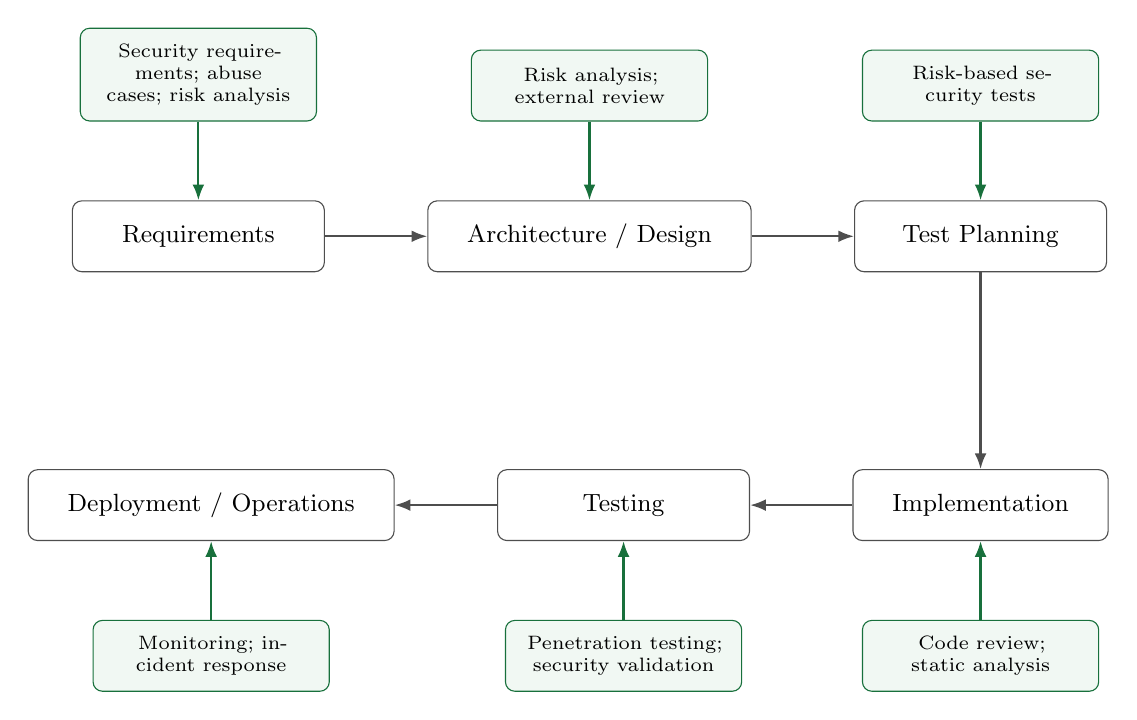
\begin{tikzpicture}[node distance=9mm and 13mm]
  % Development stages: snake layout avoids an over-wide one-line diagram.
  \node[sbox, minimum width=3.2cm] (req) {Requirements};
  \node[sbox, right=of req, minimum width=3.2cm] (design) {Architecture / Design};
  \node[sbox, right=of design, minimum width=3.2cm] (plan) {Test Planning};

  \node[sbox, below=25mm of plan, minimum width=3.2cm] (impl) {Implementation};
  \node[sbox, left=of impl, minimum width=3.2cm] (test) {Testing};
  \node[sbox, left=of test, minimum width=3.2cm] (ops) {Deployment / Operations};

  \draw[arrow] (req) -- (design);
  \draw[arrow] (design) -- (plan);
  \draw[arrow] (plan) -- (impl);
  \draw[arrow] (impl) -- (test);
  \draw[arrow] (test) -- (ops);

  \node[protectbox, above=10mm of req, text width=2.6cm, inner xsep=2mm, font=\scriptsize] (reqs) {Security requirements; abuse cases; risk analysis};
  \node[protectbox, above=10mm of design, text width=2.6cm, inner xsep=2mm, font=\scriptsize] (des) {Risk analysis; external review};
  \node[protectbox, above=10mm of plan, text width=2.6cm, inner xsep=2mm, font=\scriptsize] (tests) {Risk-based security tests};

  \node[protectbox, below=10mm of impl, text width=2.6cm, inner xsep=2mm, font=\scriptsize] (code) {Code review; static analysis};
  \node[protectbox, below=10mm of test, text width=2.6cm, inner xsep=2mm, font=\scriptsize] (pentest) {Penetration testing; security validation};
  \node[protectbox, below=10mm of ops, text width=2.6cm, inner xsep=2mm, font=\scriptsize] (monitor) {Monitoring; incident response};

  \draw[goodarrow] (reqs) -- (req);
  \draw[goodarrow] (des) -- (design);
  \draw[goodarrow] (tests) -- (plan);
  \draw[goodarrow] (code) -- (impl);
  \draw[goodarrow] (pentest) -- (test);
  \draw[goodarrow] (monitor) -- (ops);
\end{tikzpicture}
\caption{Security activities should be integrated throughout the software-development life cycle rather than added only after implementation.}
\label{fig:sdlc}
\end{figure}

The exact activity mix depends on the system, but the structural principle is stable: security requirements and risk decisions made early are cheaper to enforce than architectural flaws discovered after deployment.

\section{Authentication, Authorisation, Auditing, and Action}

A practical operational view of security groups several recurring functions:

\begin{table}[htbp]
\centering
\caption{Authentication, authorisation, auditing, and response activities.}
\label{tab:aaaa}
\begin{tabularx}{0.90\textwidth}{>{\bfseries}L{3.1cm} Y}
\toprule
\rowcolor{TableTint}
Activity & Purpose \\
\midrule
Authentication & Establish who or what a subject is. \\
Authorisation / access control & Determine which operations the subject is permitted to perform. \\
Auditing & Record and inspect security-relevant events so that violations can be detected and reconstructed. \\
Action / response & Contain incidents, recover assets, repair damage, and reduce the chance of recurrence. \\
\bottomrule
\end{tabularx}
\end{table}

These functions align with the broader sequence of \emph{prevention}, \emph{detection}, and \emph{reaction}. Prevention attempts to stop violations before they occur; detection discovers violations that bypass prevention; reaction limits damage and restores a trustworthy state.

Strong prevention does not make detection and reaction unnecessary. Perfect prevention is rarely realistic, and a system that cannot detect or respond to failure remains fragile when a preventive mechanism is bypassed.


A security policy is useful only if its intended restrictions can be stated precisely and enforced. Two practical bottlenecks follow: expressing exactly what the system should and should not permit, and implementing mechanisms that enforce those requirements either statically, before execution, or dynamically, while the system runs.

\section{Countermeasures Across the Stack}
\label{sec:countermeasures}

Countermeasures can be implemented at multiple abstraction levels. No single layer is sufficient by itself. Defensive measures also need not be purely technical: physical building security, personnel screening, legal deterrence, and law enforcement can reduce risk even though they sit outside the software stack.

At the technical level, different mechanisms address different classes of problem. Cryptography protects communication and storage against disclosure or tampering; access control constrains misbehaving users or principals; language-based mechanisms constrain programs through typing, memory safety, sandboxing, or code-based access control. The infrastructure may provide some of these mechanisms, but the software implementing the infrastructure must itself be trustworthy.

\begin{table}[htbp]
\centering
\caption{Examples of countermeasures at different abstraction levels.}
\label{tab:countermeasures}
\begin{tabularx}{\textwidth}{>{\bfseries}L{3.0cm} Y}
\toprule
\rowcolor{TableTint}
Layer & Representative mechanisms \\
\midrule
Programming / language & Safer APIs, memory-safe types, bounds checks, secure coding patterns, compiler diagnostics, static analysis, instrumentation. \\
Operating system / runtime & Sandboxing, process isolation, access control, non-executable memory, address-space randomisation. \\
Hardware & Trusted Platform Modules (TPM), protected execution support such as enclave-style mechanisms, CPU-level tracking or protection features, and memory-protection mechanisms. \\
Network / storage infrastructure & Cryptographic channels, authentication, access control, integrity protection. \\
Operational process & Monitoring, incident response, patch management, configuration review, least privilege. \\
\bottomrule
\end{tabularx}
\end{table}

A countermeasure can create new risks. For example, locking an account after a small number of failed logins reduces password-guessing opportunities but can also create a denial-of-service mechanism if an attacker deliberately triggers the lockout. Security controls therefore require their own threat analysis.

\section{Assurance and the Meaning of ``Secure''}
\label{sec:assurance}

Security is not a binary property that can normally be demonstrated by one successful test. A system can be secure relative to a stated policy and threat model while remaining vulnerable outside those assumptions. Engineering therefore requires \emph{assurance}: evidence that the chosen security goals are actually met to an appropriate level of confidence.

Useful evidence may include design review, code analysis, testing, fuzzing, penetration testing, formal verification, operational monitoring, and independent evaluation. None of these techniques is a universal proof of complete security.

The distinction between actual protection and perceived protection is also important. A mechanism can create a feeling of safety without materially reducing risk. Conversely, effective controls often impose costs in performance, convenience, usability, privacy, or operational complexity. Those costs are part of the engineering decision rather than evidence that the control is unnecessary.

\begin{keyconcept}
Secure software is not simply software that contains security features. It is software whose intended and unintended behaviors have been constrained, justified, and evaluated against an explicit threat model.
\end{keyconcept}

\section{What Secure Software Engineering Is Not}

Several common misconceptions obscure the engineering problem:

\begin{itemize}
  \item \textbf{Not a myth.} Insecure software causes concrete harm; security defects have operational consequences.
  \item \textbf{Not an arcane black art.} Exploit construction can be highly specialised, but developers know the system's intended design and can learn the mindset required to remove vulnerabilities before attackers discover them.
  \item \textbf{Not a set of features.} Adding cryptography, a security library, or a scanning tool does not automatically make an application secure. Security mechanisms can themselves be configured or used incorrectly.
  \item \textbf{Not only mathematics or cryptography.} Formal reasoning and cryptography are powerful, but they cannot compensate for an application that misuses inputs, privileges, memory, or interfaces.
  \item \textbf{Not only network or operating-system security.} A protected network path cannot repair an application-level defect, and software vulnerabilities exist even without network connectivity.
\end{itemize}

The practical goal is a learnable engineering mindset: prevent unintended functionality at every layer of the stack and gather evidence that the protections actually work.

\section{Secure Software as a Shared Responsibility}

Software security cannot be delegated entirely to cryptographers, network administrators, operating-system specialists, or security tools. Cryptography can protect data in transit and at rest while leaving application logic vulnerable. A firewall can restrict network paths while an exposed application still mishandles input. A security library can be used incorrectly.

The engineering responsibility is therefore distributed across developers, architects, operators, reviewers, and other stakeholders. The necessary mindset is learnable: identify trust boundaries, minimize attack surface, validate untrusted input, use safer abstractions, apply least privilege, and gather evidence that controls work as intended.

\section{Chapter Summary}

Secure software engineering combines precise goals, threat-aware design, safer implementation practices, layered countermeasures, and continuous evidence gathering. The central shift is from reactive patching to proactive risk management throughout the SDLC. Prevention, detection, and response complement one another, and every security mechanism must itself be evaluated for new failure modes.

% ============================================================
\chapter{Buffer Overflows and Memory Safety}
\label{chap:buffer-overflow}
% ============================================================

Buffer overflows are a concrete example of how low-level programming abstractions can become security vulnerabilities when untrusted input controls memory writes. The important lesson extends beyond one bug class: memory safety, integer representation, string conventions, and API contracts all form part of the effective security boundary of a C or C++ program.

\section{The Essence of an Out-of-Bounds Write}

Consider an array of four bytes:

\begin{lstlisting}[language=C,caption={An out-of-bounds write in C.},label={lst:oob-basic}]
char buffer[4];
buffer[4] = 'a';
\end{lstlisting}

Valid indices are \(0\) through \(3\). Writing index \(4\) exceeds the array bounds and invokes undefined behavior in C. The effect is not specified by the language: the program might appear to continue, crash, corrupt nearby data, or alter control information.

When the written value or length is influenced by an attacker, an ordinary memory-safety bug can become a vulnerability. The attacker is no longer waiting for accidental corruption; the input is chosen deliberately to shape the corrupted memory.

\begin{definitionbox}{Buffer Overflow}
A buffer overflow occurs when a program writes beyond the bounds of an allocated buffer and therefore modifies memory outside the object that was intended to receive the data.
\end{definitionbox}

A stack overflow in this context means overflowing a buffer allocated within a stack frame; a heap overflow means overflowing a dynamically allocated object. Both are instances of out-of-bounds memory access.

\section{Why C and C++ Are Exposed}

C and C++ give programmers direct control over memory layout, pointer arithmetic, allocation, and low-level strings. This control is valuable for systems programming but shifts responsibility for many safety properties to the programmer.

Common defects include:

\begin{itemize}
  \item writing past array bounds;
  \item dangling or uninitialised pointers;
  \item incorrect pointer arithmetic;
  \item double deallocation or invalid deallocation;
  \item unchecked allocation failure;
  \item integer truncation, overflow, or signedness conversion;
  \item non-terminated character arrays treated as C strings.
\end{itemize}

The security impact is especially severe for privileged services and any C/C++ code that parses data from untrusted networks, files, devices, users, or message formats.


Network daemons, browsers, wireless drivers, privileged multi-user services, parsers for downloaded or emailed files, and embedded devices with network connectivity are therefore particularly exposed. The risk follows the trust boundary: whenever attacker-controlled bytes can influence memory operations in C or C++, memory-management mistakes can become remotely or locally exploitable.

\subsection{Language-Level Bounds Checking}

One direct solution is run-time array-bounds checking. Languages and runtimes that enforce bounds and checked references can turn an out-of-range access into a controlled exception rather than silent memory corruption. Safer language designs can also reject or warn about dangerous signed/unsigned conversions, represent allocation failure through a controlled error mechanism, initialize managed memory predictably, or provide checked arithmetic where the language or API chooses to do so. C and C++ traditionally leave many of these invariants to the program for low-level control and performance. This design choice explains why memory-safety bugs have remained a recurring security problem in C/C++ code.

\section{Process Memory Layout}
\label{sec:memory-layout}

A simplified process layout is useful for reasoning about memory corruption. Program code and static data occupy lower regions, the heap typically grows toward higher addresses as dynamic allocations are made, and the call stack is commonly placed toward higher addresses and grows in the opposite direction.

\begin{figure}[htbp]
\centering
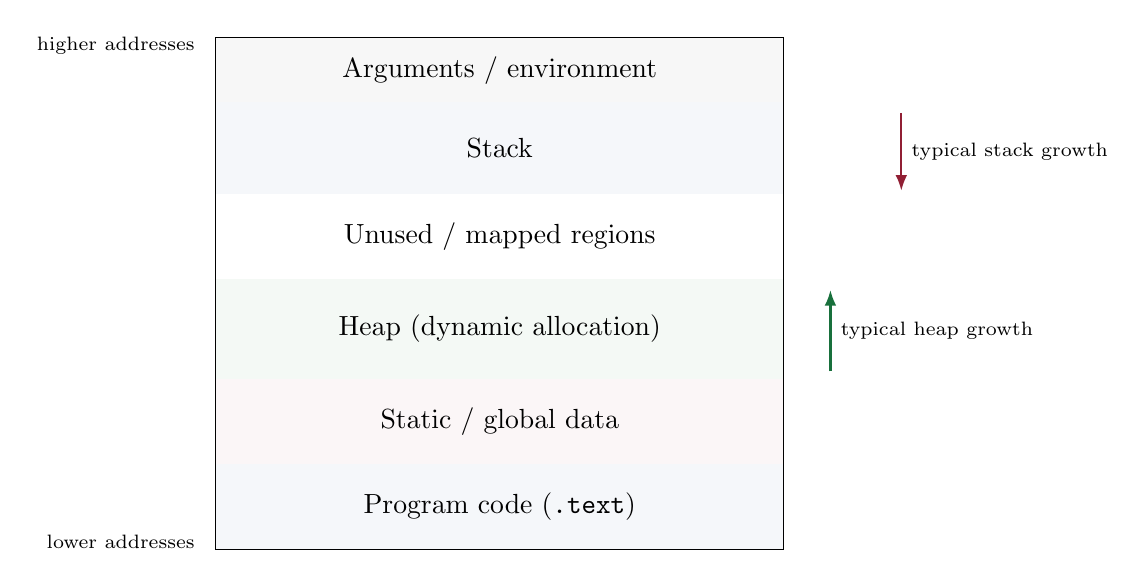
\begin{tikzpicture}[x=1cm,y=0.9cm]
  \draw[thick] (0,0) rectangle (7.2,7.2);
  \fill[SoftBlueGray] (0,0) rectangle (7.2,1.2);
  \fill[SoftRed] (0,1.2) rectangle (7.2,2.4);
  \fill[SoftGreen] (0,2.4) rectangle (7.2,3.8);
  \fill[white] (0,3.8) rectangle (7.2,5.0);
  \fill[SoftBlueGray] (0,5.0) rectangle (7.2,6.3);
  \fill[SoftGray] (0,6.3) rectangle (7.2,7.2);

  \node at (3.6,0.6) {Program code (\texttt{.text})};
  \node at (3.6,1.8) {Static / global data};
  \node at (3.6,3.1) {Heap (dynamic allocation)};
  \node at (3.6,4.4) {Unused / mapped regions};
  \node at (3.6,5.65) {Stack};
  \node at (3.6,6.75) {Arguments / environment};

  \draw[goodarrow] (7.8,2.5) -- (7.8,3.65) node[midway,right,font=\scriptsize]{typical heap growth};
  \draw[badarrow] (8.7,6.15) -- (8.7,5.05) node[midway,right,font=\scriptsize]{typical stack growth};

  \node[font=\scriptsize,anchor=east] at (-0.15,0.1) {lower addresses};
  \node[font=\scriptsize,anchor=east] at (-0.15,7.1) {higher addresses};
\end{tikzpicture}
\caption{Simplified process memory layout. Exact placement and growth direction depend on the architecture, ABI, operating system, and runtime.}
\label{fig:process-layout}
\end{figure}

\begin{remarkbox}{Model, not a universal ABI rule}
The diagram is a conceptual model. Real processes use virtual memory, shared libraries, mapped files, guard regions, thread stacks, and platform-specific layouts; heap and stack growth directions are not language guarantees.
\end{remarkbox}

\section{Stack Frames and Control-Flow Corruption}
\label{sec:stack-overflow}

A function call usually creates an activation record, or stack frame, containing local variables and control data used to resume the caller. A local array can therefore be adjacent to saved state such as a return address, depending on compiler and ABI conventions.

Consider:

\begin{lstlisting}[language=C,caption={Unbounded input into a stack buffer.},label={lst:gets-stack}]
void f(int x) {
    char buf[8];
    gets(buf);       /* unsafe: no destination bound */
}
\end{lstlisting}

The obsolete \texttt{gets} function has no way to know the capacity of \texttt{buf}. An input longer than the buffer can overwrite adjacent memory.

\begin{figure}[htbp]
\centering
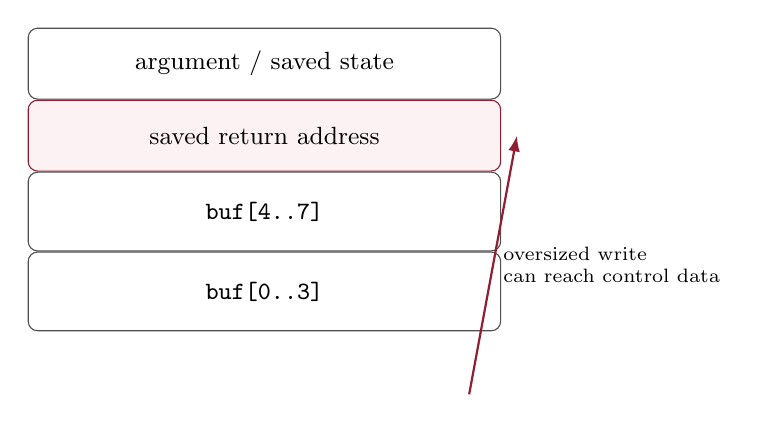
\begin{tikzpicture}[node distance=0mm]
  \node[sbox, minimum width=6.0cm, minimum height=9mm] (arg) {argument / saved state};
  \node[threatbox, below=0mm of arg, minimum width=6.0cm, minimum height=9mm] (ret) {saved return address};
  \node[sbox, below=0mm of ret, minimum width=6.0cm, minimum height=10mm] (buf2) {\texttt{buf[4..7]}};
  \node[sbox, below=0mm of buf2, minimum width=6.0cm, minimum height=10mm] (buf1) {\texttt{buf[0..3]}};

  \draw[badarrow] ($(buf1.south)+(2.6,-0.8)$) -- ($(ret.east)+(0.2,0)$) node[midway,right,font=\scriptsize,align=left]{oversized write\\can reach control data};
\end{tikzpicture}
\caption{Simplified stack-frame model. An oversized write to a local buffer may reach adjacent control data, including a saved return address.}
\label{fig:stack-overflow}
\end{figure}

Practical exploitation depends on many details: the exact stack layout, where attacker-controlled bytes reside, whether the attacker can predict addresses, which bytes can appear in the input, and whether corrupted values are used before the function returns. The vulnerability, however, exists before exploit reliability is considered: the program has already lost memory safety.

\section{Unsafe String Handling}
\label{sec:unsafe-strings}

C strings are arrays of \texttt{char} terminated by a zero byte. Because the length is not stored as part of the string type, every operation depends on correct termination and sufficient destination capacity.

\subsection{Never Use \texttt{gets}}

The correct conclusion is stronger than ``be careful with \texttt{gets}'': the function is intrinsically unsafe because its interface contains no destination-size parameter. It was removed from the C standard in C11.

A bounded read such as

\begin{lstlisting}[language=C]
char buf[20];
if (fgets(buf, sizeof buf, stdin) == NULL) {
    /* handle EOF or error */
}
\end{lstlisting}

at least communicates the capacity of the destination. The caller must still handle truncation and newline semantics correctly.

\subsection{\texttt{strcpy}, \texttt{strncpy}, and Termination}

\texttt{strcpy(dest, src)} assumes that \texttt{dest} is large enough and that \texttt{src} is null-terminated. If either assumption fails, behavior is unsafe.

Replacing \texttt{strcpy} mechanically with \texttt{strncpy} does not automatically make the code correct. If the source length is at least the requested bound, \texttt{strncpy} does not append a null terminator. A defensive pattern for a fixed-size character array is therefore

\begin{lstlisting}[language=C,caption={One bounded-copy pattern for a fixed-size destination.}]
strncpy(dest, src, sizeof dest - 1);
dest[sizeof dest - 1] = '\0';
\end{lstlisting}

This prevents an unterminated destination but may silently truncate input. Whether truncation is acceptable is an application-level decision, not merely a memory-safety decision.

\begin{examplebox}{Why \texttt{strncpy} can still fail}
If \texttt{src} has capacity 9 and receives the nine visible characters of \texttt{"www.ru.nl"}, there is no remaining byte for the terminating \texttt{'\textbackslash0'}. Treating that array as a C string later can make a function such as \texttt{strcpy} read beyond the array until an unrelated zero byte happens to be encountered.
\end{examplebox}

\subsection{The \texttt{strncat} Size Parameter}

The third parameter of \texttt{strncat(dest, src, n)} is the maximum number of characters to append from \texttt{src}; it is not the total capacity of \texttt{dest}. Correct use requires computing the remaining space after the current destination length and reserving one byte for the terminator.

\section{Length Fields, Integer Conversion, and Allocation Size}
\label{sec:integer-errors}

Memory-safety failures are often enabled by integer errors that occur before the final out-of-bounds access.

\subsection{Signed Length from Untrusted Input}

Consider a length read from an untrusted file descriptor:

\begin{lstlisting}[language=C,caption={Unsafe use of an unvalidated length field.}]
char *buf;
int len;

read(fd, &len, sizeof len);
buf = malloc(len);
read(fd, buf, len);
\end{lstlisting}

A negative \texttt{len} is problematic because allocation and I/O APIs use unsigned size types. Implicit conversion can transform a negative integer into a very large positive size. The code also fails to check return values from \texttt{read} and \texttt{malloc}.

Attempting to ``fix'' termination by allocating \texttt{len} bytes, reading \texttt{len+1}, and writing \texttt{buf[len] = '\textbackslash0'} introduces explicit off-by-one writes. Correct code must validate the length, account for any terminator in the allocation, and verify every operation.

\subsection{Narrowing a String Length}

The following pattern is also unsafe:

\begin{lstlisting}[language=C,caption={Narrowing a string length before a bounds check.}]
#define MAX_BUF 256

void BadCode(char *input) {
    short len;
    char buf[MAX_BUF];

    len = strlen(input);
    if (len < MAX_BUF)
        strcpy(buf, input);
}
\end{lstlisting}

\texttt{strlen} returns \texttt{size\_t}, which can represent values much larger than \texttt{short}. Converting a long input length to \texttt{short} can change the value before the comparison. The bounds check then reasons about the truncated value rather than the true source length.

\subsection{Multiplication Overflow in Allocation}

A request to allocate an array of \(n\) objects conceptually requires

\begin{equation}
\text{bytes}=n\cdot \operatorname{sizeof}(T).
\label{eq:alloc-size}
\end{equation}

If this multiplication overflows the size type, the allocated block can be smaller than required even though later code iterates over all \(n\) elements. Robust code must validate both the element count and the multiplication used to compute the allocation size.

\section{Bytes versus Characters}

Size units are part of the API contract. For narrow character arrays, a byte count and character count coincide. For wide-character arrays they do not.

If a function such as \texttt{\_snwprintf} expects a count of \texttt{wchar\_t} elements, passing \texttt{sizeof(buffer)} supplies a byte count instead. On a platform where \texttt{wchar\_t} occupies more than one byte, the apparent bound is too large. ANSI/Unicode size mismatches of this form are historically important because they have enabled real buffer-overflow vulnerabilities, including the class of error associated with Code Red. The general rule is to distinguish \emph{object count} from \emph{byte count} explicitly.

\section{Sentinel and Loop-Condition Errors}

Bounds checks can be correct in isolation and still fail when later code searches for a sentinel that may not exist. For example, code that copies characters until the first slash in a URL must also stop at the string terminator. Otherwise the loop can continue past the validated input length while looking for a delimiter that is absent.

Order matters when conditions contain side effects such as \texttt{*url++}. Advancing a pointer before testing whether the end has been reached can invalidate an otherwise sensible boundary check. The safer design is to separate pointer advancement from the stopping conditions so each operation has an explicit precondition.

\section{Format String Vulnerabilities}
\label{sec:format-strings}

A format string is executable metadata: conversion specifiers tell a function such as \texttt{printf} how to interpret additional arguments. Passing attacker-controlled data as the format itself therefore mixes data with instructions.

\begin{lstlisting}[language=C,caption={Vulnerable and safe treatment of untrusted output text.}]
/* vulnerable */
printf(argv[1]);

/* safe data treatment */
printf("%s", argv[1]);
\end{lstlisting}

Specifiers such as \texttt{\%x} may expose unintended values from the variadic argument interpretation, while \texttt{\%n} can write the number of characters printed so far through a pointer interpreted from the argument list. Exploitation does not require a conventional buffer overflow; the vulnerability can provide unintended reads or writes directly.

\begin{keyconcept}
A format-string bug violates the ``do not mix data and control'' principle. The secure pattern is to keep the format string constant and pass untrusted text only as data arguments.
\end{keyconcept}

\section{Runtime Countermeasures}
\label{sec:runtime-mitigations}

Runtime defenses reduce exploitability even when a memory-safety bug remains.

\subsection{Non-Executable Memory and Address Randomisation}

Non-executable data memory prevents a common class of attacks from simply placing new machine code in writable memory and executing it. Address-space layout randomisation (ASLR) makes important addresses less predictable across executions. Instruction-set randomisation is another conceptual defense: code is interpreted through a randomised encoding so injected instructions are unlikely to have the intended meaning, although efficient deployment requires suitable support. Compiler transformations may also obscure or randomise memory addresses. These mechanisms raise the cost of exploitation but do not repair the underlying out-of-bounds write and do not, by themselves, prevent heap corruption.

\subsection{Stack Canaries}

A stack canary is a value placed between vulnerable local data and critical control information. The function checks the canary before returning. A simple sequential overwrite that reaches the saved return address is therefore expected to modify the canary first.

\begin{figure}[htbp]
\centering
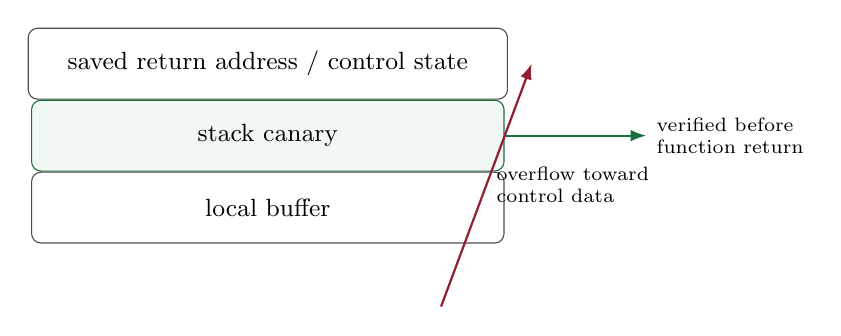
\begin{tikzpicture}[node distance=0mm]
  \node[sbox, minimum width=6cm] (saved) {saved return address / control state};
  \node[protectbox, below=0mm of saved, minimum width=6cm] (canary) {stack canary};
  \node[sbox, below=0mm of canary, minimum width=6cm] (buf) {local buffer};

  \draw[badarrow] ($(buf.south)+(2.2,-0.8)$) -- ($(saved.east)+(0.3,0)$) node[midway,right,font=\scriptsize,align=left]{overflow toward\\control data};
  \draw[goodarrow] (canary.east) -- ++(1.8,0) node[right,font=\scriptsize,align=left]{verified before\\function return};
\end{tikzpicture}
\caption{Stack-canary principle. A sequential overwrite toward control data is expected to alter the canary before reaching the saved return state.}
\label{fig:canary}
\end{figure}

Randomised canaries make it harder for an attacker to reproduce the expected value. Variants can bind the canary to control data, for example by XORing a random value with the saved return address, or include string-termination bytes so common string-copy operations cannot reproduce the value easily. Canaries remain a mitigation rather than a proof of memory safety: a memory disclosure may reveal the canary, an attacker may preserve or reconstruct it, non-sequential writes may bypass it, the protected ``master'' value must itself be stored safely, and heap corruption is outside its direct scope.

\subsection{Defense in Depth and Additional Runtime Protections}

Several historical defenses extend the canary idea. \emph{PointGuard} protects selected pointer values, including function pointers, using encoded or guarded representations. IBM's \emph{ProPolice / Stack Smashing Protection (SSP)} combines stack protection with reordering of stack objects to reduce the chance that an overflowing buffer immediately reaches sensitive state. \emph{StackShield} separates or checks return-address information and can impose additional restrictions on control transfers.

These mechanisms illustrate a broader defense-in-depth strategy: compilers and runtimes can reorder stack objects, protect selected pointers, insert bounds instrumentation, or add control-flow checks. Their purpose is to reduce exploit reliability or impact. None is perfect; protected return addresses do not guarantee the integrity of other stack data, clever writes may avoid a canary, and stack-focused defenses do not remove heap overflows. Multiple independent defenses are therefore stronger than reliance on a single mechanism.

\section{Prevention and Detection}
\label{sec:prevention-detection}

The strongest preventive strategy is to avoid unsafe memory management when the application does not require it. Memory-safe languages can enforce array bounds and prevent many classes of dangling-pointer and raw-memory errors by construction.

When C or C++ is necessary, security depends on disciplined interfaces and multiple forms of analysis.

\subsection{High-Risk C Interfaces}

Some C library interfaces deserve special scrutiny because their contracts make size mistakes easy. The following classification groups interfaces by how readily their contracts can lead to dangerous size or format mistakes; actual risk still depends on how each function is used and on whether lengths, formats, and termination are validated.

\begin{table}[htbp]
\centering
\small
\caption{Risk-oriented classification of C interfaces that require careful use.}
\label{tab:dangerous-c}
\begin{tabularx}{\textwidth}{>{\bfseries}L{2.6cm} Y}
\toprule
\rowcolor{TableTint}
Risk group & Functions highlighted for review \\
\midrule
Extreme & \texttt{gets} \\
High & \texttt{strcpy}, \texttt{strcat}, \texttt{sprintf}, \texttt{scanf}, \texttt{sscanf}, \texttt{fscanf}, \texttt{vfscanf}, \texttt{vsscanf}, \texttt{streadd}, \texttt{strecpy}, \texttt{strtrns}, \texttt{realpath}, \texttt{syslog}, \texttt{getenv}, \texttt{getopt}, \texttt{getopt\_long}, \texttt{getpass} \\
Moderate & \texttt{getchar}, \texttt{fgetc}, \texttt{getc}, \texttt{read}, \texttt{bcopy} \\
Lower, but still contract-sensitive & \texttt{fgets}, \texttt{memcpy}, \texttt{snprintf}, \texttt{strccpy}, \texttt{strcadd}, \texttt{strncpy}, \texttt{strncat}, \texttt{vsnprintf} \\
\bottomrule
\end{tabularx}
\end{table}

The point is not that a function name alone determines vulnerability. Even bounded interfaces can be misused when the bound has the wrong unit or meaning, as shown by \texttt{strncat}, wide-character APIs, and incorrect \texttt{sizeof} usage.

\subsection{Static and Dynamic Buffer Strategies}

Fixed-size buffers make resource use predictable but are easy to size incorrectly; silently truncating input can also change program semantics. Dynamically growing buffers avoid a fixed capacity but introduce allocation failure and out-of-memory behavior that must itself fail safely. Choosing dynamic storage therefore moves, rather than eliminates, part of the security problem.

\subsection{Safer String Libraries and Abstractions}

Historical and platform-specific libraries have attempted to make unsafe string handling harder. Their details vary, but they illustrate useful API design principles.

\begin{table}[htbp]
\centering
\caption{Examples of safer string-handling approaches and their intended improvement.}
\label{tab:string-libraries}
\begin{tabularx}{\textwidth}{>{\bfseries}L{3.2cm} Y}
\toprule
\rowcolor{TableTint}
Mechanism & Security idea \\
\midrule
\texttt{libsafe} & Replaces selected unsafe C library operations and attempts to prevent writes beyond the current stack frame. \\
\texttt{libverify} & Extends the idea by retaining protected copies of return addresses for comparison. \\
\texttt{strlcpy}/\texttt{strlcat} & Take the total destination-buffer size rather than a ``maximum characters copied'' interpretation, making the capacity contract easier to use consistently. \\
GLib \texttt{GString} & Provides dynamically growing null-terminated strings; allocation failure still requires a safe failure strategy. \\
Microsoft \texttt{Strsafe} family & Uses destination-size-aware interfaces intended to guarantee termination under their documented contracts. \\
C++ \texttt{std::string} & Encapsulates dynamic string storage, while conversions back to raw C-string pointers reintroduce lower-level interface assumptions. \\
\bottomrule
\end{tabularx}
\end{table}

\begin{table}[htbp]
\centering
\caption{Memory-safety defenses at different stages of development and execution.}
\label{tab:memory-defense}
\begin{tabularx}{\textwidth}{>{\bfseries}L{3.0cm} Y}
\toprule
\rowcolor{TableTint}
Stage & Useful defenses \\
\midrule
Design & Minimise attack surface, choose safer abstractions, isolate privileged components, define input bounds and failure behavior. \\
Implementation & Prefer bounded APIs, validate lengths and integer conversions, check allocation and I/O results, enable compiler diagnostics and hardening. \\
Testing & Boundary-value tests, fuzzing, sanitizers, code review, dynamic analysis. \\
Pre-release analysis & Static analysis, specialised memory-safety tools, targeted penetration testing, formal verification for high-assurance components. \\
Runtime & ASLR, non-executable memory, stack protection, sandboxing, least privilege, monitoring. \\
\bottomrule
\end{tabularx}
\end{table}

Fuzz testing is particularly useful for parsers and input-handling code because it systematically exposes the program to malformed or unusual inputs that ordinary functional tests may never generate. Static analysis and code review complement fuzzing by searching for unsafe data flows and API use before execution.

Historically used source-scanning and static-analysis tools include RATS, Flawfinder, ITS4, Deputy, Splint, and Microsoft's PREfix/PREfast family. Tool names and capabilities evolve, but the engineering role is stable: automated analysis searches for dangerous calls, suspicious data flows, type or bounds inconsistencies, and other patterns before release. Code review remains complementary because tools cannot infer every application-specific security invariant.

At the most demanding end of static reasoning, program verification attempts to prove memory-management properties mathematically, for example using Hoare-style assertions or deductive verification. Such verification can provide much stronger evidence than testing for the properties actually proved, but it is labour-intensive and depends on the correctness and completeness of the specification.

\section{Reducing the Attack Surface}

A vulnerability cannot be exploited through a feature that is not present or reachable. Removing unnecessary services, disabling unused functionality, limiting privileges, and narrowing exposed interfaces all reduce the number of possible attack paths.

This principle is especially valuable when complete defect elimination is unrealistic. Reducing attack surface changes the environment in which remaining vulnerabilities can be reached.

\section{General Lessons from Buffer Overflows}

Buffer overflows expose three broader security failures:

\begin{enumerate}
  \item \textbf{Insufficient input validation.} External sizes, indices, delimiters, and encodings must be validated before they influence memory operations.
  \item \textbf{Mixing data and control.} A stack frame can place ordinary data near control state; format strings can interpret attacker-controlled bytes as instructions for the formatting engine.
  \item \textbf{Over-trusting abstractions.} Procedure calls, string APIs, integer types, and allocation routines provide useful abstractions, but low-level languages do not always enforce the assumptions programmers make about them.
\end{enumerate}

The deeper engineering lesson is that attackers often search for gaps between an abstraction's convenient mental model and the exact behavior enforced by the language, compiler, runtime, and hardware.

\section{Recommended Follow-up}

For deeper study of secure C/C++ programming and memory-safety defenses, useful themes include secure coding guidelines, dynamic buffer-overflow prevention, static analysis, fuzzing, and formal verification. One source explicitly associated with this topic is John Wilander and Mariam Kamkar's comparison of publicly available tools for dynamic buffer-overflow prevention.

\section{Chapter Summary}

Buffer overflows arise when software loses control of memory boundaries. In C and C++, unsafe string handling, unchecked lengths, integer conversion, allocation-size overflow, delimiter logic, and format strings can all create or amplify memory corruption. Runtime mitigations such as ASLR, non-executable memory, and stack canaries reduce exploitability but do not remove the bug. The strongest approach combines safer abstractions, explicit validation, development-time analysis, runtime hardening, and a reduced attack surface.

% ============================================================
\chapter*{Quick Review}
\addcontentsline{toc}{chapter}{Quick Review}
\markboth{Quick Review}{}
% ============================================================

\begin{enumerate}
  \item Software security concerns both the protection provided by software and the risks introduced by software behavior.
  \item Functional properties state what a system should do; security properties also constrain what it must not do under hostile input.
  \item A threat model identifies relevant attackers, capabilities, assets, and prohibited outcomes.
  \item CIA stands for confidentiality, integrity, and availability. Authentication is separate from availability.
  \item A bug or flaw is not automatically a vulnerability; the weakness must have security consequences under the relevant threat model.
  \item An exploit is a concrete way to trigger a vulnerability; malware is malicious software and may use one or more exploits.
  \item Risk arises when threats can exploit vulnerabilities and harm assets; countermeasures are introduced to reduce that risk.
  \item Security depends on the full software stack, including libraries, runtimes, operating systems, build tools, and hardware interfaces.
  \item The trusting-trust problem shows why source review alone cannot establish trust in a compromised build chain.
  \item Security work belongs throughout the SDLC: requirements, design, implementation, testing, deployment, and operation.
  \item Prevention, detection, and response are complementary; strong prevention does not eliminate the need for the other two.
  \item A security mechanism can create new vulnerabilities, so countermeasures themselves require threat analysis.
  \item An out-of-bounds write in C invokes undefined behavior and may corrupt ordinary data or control state.
  \item A stack buffer overflow can reach saved control information when the layout places it adjacent to a local array.
  \item \texttt{gets} is inherently unsafe because it has no destination-size parameter.
  \item \texttt{strncpy} is not a drop-in ``safe strcpy''; it may leave the destination unterminated and can silently truncate data.
  \item \texttt{strncat}'s bound limits appended characters, not total destination capacity.
  \item Integer truncation, signedness conversion, and allocation-size multiplication can turn apparently checked lengths into unsafe memory operations.
  \item Format-string vulnerabilities arise when untrusted data is used as a format rather than passed as data to a constant format string.
  \item ASLR, non-executable memory, and stack canaries reduce exploitability but do not repair memory-safety defects.
  \item Fuzzing, static analysis, code review, compiler diagnostics, and sanitizers complement one another because each detects different classes of failure.
  \item Reducing attack surface limits the paths through which remaining vulnerabilities can be reached.
  \item Memory-safe languages can eliminate entire categories of errors by enforcing invariants that C and C++ leave to the programmer.
  \item Security is relative to a threat model and evidence; the absence of a known attack is not proof that no vulnerability exists.
  \item Security theater improves perceived protection without necessarily reducing the relevant risk; effective controls must be evaluated against the actual threat model.
  \item Design flaws, implementation bugs, configuration mistakes, user choices, and unforeseen feature interactions can all become sources of vulnerability.
  \item Defending against exploit activity, threat actors, and underlying vulnerabilities are related but distinct security tasks.
  \item Hardware and platform mechanisms such as TPM-style roots of trust, protected execution, sandboxing, and memory protection complement application-level controls.
  \item Instruction-set randomisation, pointer protection, ProPolice/SSP-style stack protection, and StackShield-like mechanisms illustrate the historical arms race between memory-corruption exploits and mitigations.
  \item Safer libraries reduce API misuse only when their size, termination, and failure contracts are understood correctly.
  \item Formal verification can establish strong properties for a specified model, but the cost and specification burden make it one component of assurance rather than a universal solution.
\end{enumerate}

\end{document}
